% !TEX recipe = pdflatex x2 (slides)
\documentclass[aspectratio=169,11pt]{beamer}
\usetheme{Madrid}
\usepackage[utf8]{inputenc}
\usepackage[T1]{fontenc}
\usepackage{amsmath,amssymb}
\usepackage{booktabs}
\graphicspath{{../figures/}}

\setbeamertemplate{navigation symbols}{}
\definecolor{omegacol}{RGB}{217,119,43}
\newcommand{\sdtw}{\mathrm{dtw}_\gamma}
\newcommand{\minop}{\mathop{\mathrm{min}^\gamma}}
\newcommand{\ours}[1]{{\color{omegacol}#1}}

\title[Soft-DTW]{Soft-DTW: a Differentiable Loss Function for Time-Series}
\subtitle{Reproduction of Cuturi \& Blondel (ICML 2017) and an extension: soft-DTW with a warping penalty}
\author[Borrego, Tibau]{Pablo Borrego \and Pol Tibau}
\institute[MVA]{MVA -- Machine Learning for Time Series}
\date{December 2026}

\begin{document}

% ----------------------------------------------------------------------
\begin{frame}
\titlepage
\note{Our project is on soft-DTW (Cuturi and Blondel, ICML 2017). We re-implemented it from scratch, reproduced its four experiments and added an extension: a penalty on time warping. The talk follows the report: problem, method, data and reproduction, then our extension.}
\end{frame}

% ----------------------------------------------------------------------
\section{The problem}
\begin{frame}{Comparing series that are shifted or stretched in time}
\begin{columns}[T]
\begin{column}{0.48\textwidth}
\begin{block}{DTW: the cheapest monotone alignment}
\[
\mathrm{dtw}(x,y)=\min_{A\in\mathcal A_{n,m}}\langle A,\Delta(x,y)\rangle
\]
with costs $\delta_{i,j}=\|x_i-y_j\|^2$; computed by dynamic programming in $O(nm)$.
\end{block}
\end{column}
\begin{column}{0.48\textwidth}
\begin{block}{DTW it is not differentiable}
The minimum jumps from one path to another when $x$ changes: DTW has kinks and cannot be used directly as a training loss.
\end{block}
\end{column}
\end{columns}
\vspace{0.2cm}
\centering
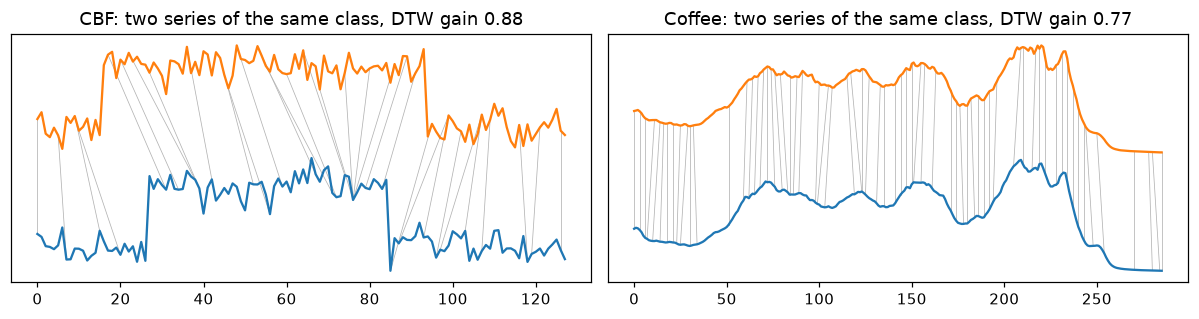
\includegraphics[width=0.8\textwidth]{data_alignment.png}\\

\note{Two series of the same class often have the same shape but are shifted or stretched in time. DTW finds the cheapest monotone alignment between their time steps; its value is the cost of that alignment, computed by dynamic programming in O(nm). But the minimum is not differentiable: when x changes the optimal path jumps, so DTW cannot be used as a loss.}
\end{frame}

% ----------------------------------------------------------------------
\section{Method}
\begin{frame}{Soft-DTW replaces the minimum by a soft-minimum}
\begin{columns}[T]
\begin{column}{0.5\textwidth}
\[
\minop(a_1,\dots,a_k)=-\gamma\log\sum_{l} e^{-a_l/\gamma}
\]
\[
\sdtw(x,y)=\minop_{A\in\mathcal A_{n,m}}\langle A,\Delta(x,y)\rangle
\]
\begin{itemize}
\item $\gamma\to0$ recovers DTW
\item $\gamma>0$: smooth in $x$
\end{itemize}
\end{column}
\begin{column}{0.46\textwidth}
\begin{block}{Its gradient has a meaning}
\[
\nabla_x\sdtw=\sum_{i,j}e_{i,j}\,\frac{\partial\delta_{i,j}}{\partial x},\qquad E=\mathbb E_\gamma[A]
\]
$e_{i,j}$: share of all alignments that match $x_i$ with $y_j$, each alignment $A$ counting with weight $e^{-\mathrm{cost}_A/\gamma}$.
\end{block}
\end{column}
\end{columns}
\vspace{0.1cm}
\centering
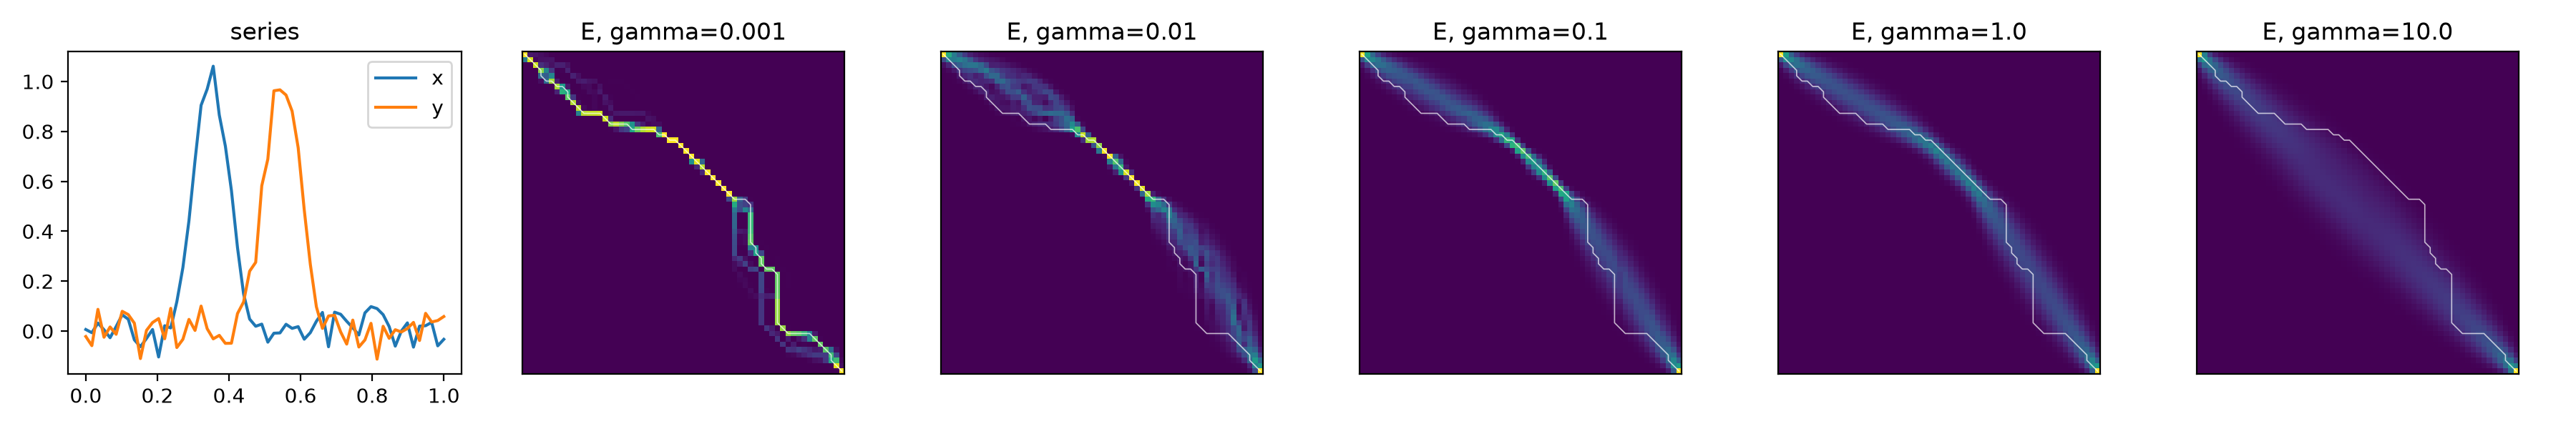
\includegraphics[width=0.84\textwidth]{E_vs_gamma.png}\\
{\scriptsize $E$ for increasing $\gamma$: the DTW path (white) becomes a diffuse band.}
\note{Soft-DTW keeps everything from DTW but replaces the minimum by a soft-minimum with smoothing parameter gamma: it averages over all alignments, the cheap ones weighing much more. Gamma to zero recovers DTW; for gamma positive it is smooth. Its gradient is weighted by E, the expected alignment: the probability that a path goes through each cell. For small gamma E is the DTW path; as gamma grows it spreads into a band.}
\end{frame}

\begin{frame}{Two $O(nm)$ recursions, implemented from scratch}
\begin{columns}[T]
\begin{column}{0.32\textwidth}
\begin{block}{Forward (Alg.\ 1)}
Bellman's recursion: $r_{i,j}=\delta_{i,j}+\minop$ of its 3 neighbours $r_{i-1,j-1}$, $r_{i-1,j}$, $r_{i,j-1}$. Value: $r_{n,m}$.
\end{block}
\end{column}
\begin{column}{0.32\textwidth}
\begin{block}{Backward (Alg.\ 2)}
From $(n,m)$ back to $(1,1)$, each cell collects $e_{i,j}$ from its 3 successors: $E$ and the gradient.
\end{block}
\end{column}
\begin{column}{0.32\textwidth}
\begin{block}{Gradient}
Chain rule through the costs: $\nabla_{x_i}\sdtw=\sum_j e_{i,j}\,2(x_i-y_j)$. Same $O(nm)$ cost as the value.
\end{block}
\end{column}
\end{columns}
\vspace{0.2cm}
{\small\textbf{Our implementation}}
\begin{columns}[T]
\begin{column}{0.32\textwidth}
\begin{block}{Numba core}
Both recursions compiled with Numba, soft-min computed stably (log-sum-exp). $0.3$ ms for $n=m=64$.
\end{block}
\end{column}
\begin{column}{0.32\textwidth}
\begin{block}{PyTorch loss}
Usable in any network, with a hand-written backward: autograd through the recursion is $2500\times$ slower.
\end{block}
\end{column}
\begin{column}{0.32\textwidth}
\begin{block}{Verified}
For $n,m\le5$, listing every alignment gives the same value and $E$ (error $<10^{-10}$); gradients match finite differences.
\end{block}
\end{column}
\end{columns}
\note{Both the value and the gradient come from two O(nm) recursions. The forward pass is Bellman's recursion with the soft-minimum; the backward pass goes from the end to the start and gives E. We implemented both from scratch and checked them against brute-force enumeration of every alignment and finite differences. The hand-written backward matters: it is three orders of magnitude faster than autograd.}
\end{frame}

% ----------------------------------------------------------------------
\section{Data}
\begin{frame}{Data}
\begin{columns}[T]
\begin{column}{0.38\textwidth}
\begin{block}{The datasets}
\begin{itemize}
\item 13 datasets of the UCR archive (the paper used 79)
\item ECG, motion, shapes, power demand, synthetic
\item Lengths 24 to 512; 2 to 60 classes
\end{itemize}
\end{block}
\end{column}
\begin{column}{0.58\textwidth}
\begin{block}{Do they need DTW?}
\textbf{Question:} are two series of the same class misaligned in time?\\[0.15cm]
\textbf{Test:} compare their distance before and after aligning them:
\[
\text{DTW gain}=1-\frac{\mathrm{dtw}(x,y)}{\|x-y\|^2}
\]
= share of the distance that disappears once aligned.\\[0.15cm]
\textbf{Answer:} \textbf{48--96\%} on every dataset, so warping matters for all of them.
\end{block}
\end{column}
\end{columns}
\note{We use 13 datasets of the UCR archive, of several domains, lengths and numbers of classes; the paper used 79. Before using DTW we checked that the data need it: we take pairs of series of the same class and compare their Euclidean distance with their DTW distance. The DTW gain is the share of the distance that disappears once the series are aligned. It is between 48 and 96 percent on every dataset, so in all of them a large part of the difference between series of the same class is just misalignment. Some datasets have global shifts, like CBF or Trace; others are globally aligned but locally stretched, like Coffee or Plane.}
\end{frame}

% ----------------------------------------------------------------------
\section{Reproduction}
\begin{frame}{Barycenters and $k$-means}
\centering\small
\begin{tabular}{lcccc}
\toprule
\% datasets where soft-DTW beats DBA & $\gamma=1$ & $\gamma=0.1$ & $\gamma=0.01$ & $\gamma=0.001$\\
\midrule
Barycenters, random init & 58 (41) & 92 (94) & 100 (100) & 100 (97)\\
Barycenters, Euclidean-mean init & 8 (4) & 25 (47) & 75 (80) & 100 (90)\\
$k$-means, random init & 10 (16) & 50 (25) & 70 (60) & 90 (77)\\
$k$-means, Euclidean init & 10 (29) & 10 (24) & 60 (55) & 90 (69)\\
\bottomrule
\end{tabular}\\[0.05cm]
{\scriptsize Ours (12 datasets for barycenters, 10 for $k$-means) vs the paper (79) in parentheses. All scored with the hard DTW loss.}
\vspace{0.2cm}
\begin{itemize}\small
\item From a random start, the soft-DTW barycenter has a \textbf{14\% lower} DTW loss than DBA's (74\% lower on Plane).
\item From the Euclidean mean, it is only \textbf{3\% lower}.
\item With $\gamma=0.001$ it takes \textbf{14 times} as long as DBA to compute.
\end{itemize}
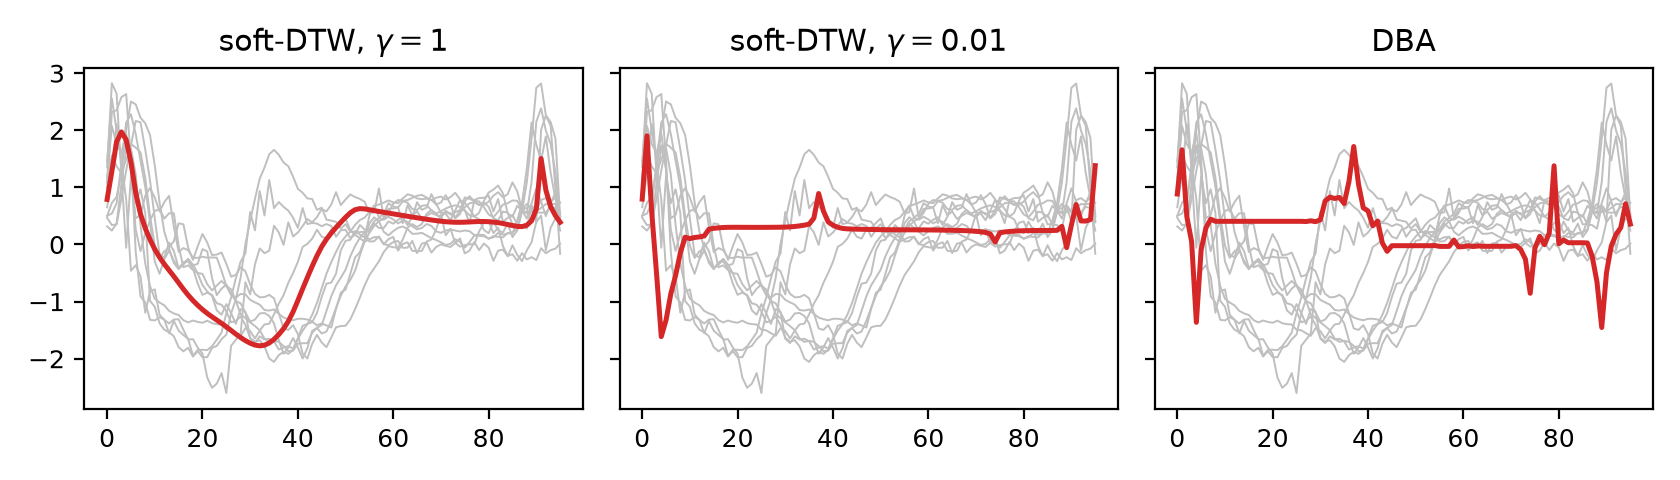
\includegraphics[width=0.48\textwidth]{barycenters_ECG200_slides.png}
\note{As in the paper we compare soft-DTW barycenters with DBA under the hard DTW loss. The win rates follow the paper: small gamma beats DBA almost always, gamma 1 rarely. But the paper only reports win rates: the gain is large only from a random start; from the Euclidean mean it is about 3 percent, and gamma 0.001 costs 14 times DBA's time.}
\end{frame}

\begin{frame}{Nearest centroid}
\begin{columns}[c]
\begin{column}{0.58\textwidth}
\centering\small
\begin{tabular}{lcc}
\toprule
 & Ours & Paper\\
\midrule
\% datasets where soft-DTW $\ge$ DBA & 83 & 75\\
Mean accuracy, DBA & 0.81 & --\\
Mean accuracy, soft-DTW & 0.86 & --\\
\bottomrule
\end{tabular}\\[0.05cm]
{\scriptsize Ours: 12 datasets, 3 random splits; paper: 79 datasets.}
\vspace{0.3cm}
\begin{itemize}\small
\item Each class is represented by the barycenter of its training series; a new series gets the class of the \textbf{closest centroid}.
\item $\gamma$ is chosen on a validation split.
\item Soft-DTW centroids classify \textbf{at least as well} as DBA's on 83\% of the datasets: better barycenters represent the class better.
\end{itemize}
\end{column}
\begin{column}{0.38\textwidth}
\centering
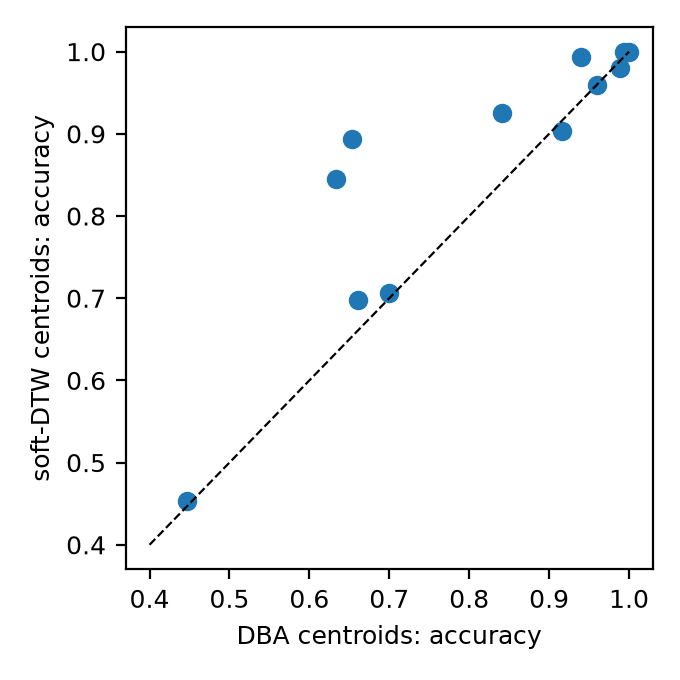
\includegraphics[width=\textwidth]{nearest_centroid_slides.png}\\
{\scriptsize One point per dataset; above the diagonal, soft-DTW wins.}
\end{column}
\end{columns}
\note{The third experiment of the paper uses barycenters to classify: each class is represented by the barycenter of its training series, and a new series takes the class of the closest one. It measures indirectly how well a barycenter represents its class. We reproduce the result: soft-DTW centroids classify at least as well as DBA's on 83 percent of the datasets, the paper had 75, with a mean accuracy of 0.86 against 0.81. In the plot each point is a dataset; above the diagonal soft-DTW wins.}
\end{frame}

\begin{frame}{Forecasting}
An MLP sees the first 60\% of a series and predicts the rest, trained with the Euclidean loss or soft-DTW, from scratch or from the Euclidean network. Average rank over 13 datasets (1 = best; paper in parentheses):
\vspace{0.2cm}
\begin{center}\small
\begin{tabular}{lccccc}
\toprule
Test metric, init & Euclidean & $\gamma=1$ & $\gamma=0.1$ & $\gamma=0.01$ & $\gamma=0.001$\\
\midrule
DTW, from scratch & 3.69 (3.46) & 3.92 (3.55) & 2.31 (3.33) & 2.23 (2.79) & 2.85 (1.87)\\
DTW, from Euclidean & 3.92 (4.21) & 4.46 (3.96) & 2.85 (3.42) & 2.08 (2.12) & 1.69 (1.29)\\
Euclidean, from scratch & 1.31 (1.05) & 1.69 (2.41) & 3.46 (3.42) & 4.00 (4.13) & 4.54 (3.99)\\
\bottomrule
\end{tabular}
\end{center}
\begin{columns}[T]
\begin{column}{0.48\textwidth}
\begin{block}{What the table shows}
Each loss wins on its own metric: soft-DTW with a small $\gamma$ ranks best in DTW, the Euclidean loss in Euclidean distance. From the Euclidean network, the smaller $\gamma$, the better, as in the paper.
\end{block}
\end{column}
\begin{column}{0.48\textwidth}
\begin{block}{Outliers}
From scratch, $\gamma=0.001$ is unstable: on Coffee the test DTW is $3.2\times$ the Euclidean network's. On ShapesAll the forecast degenerates (next slide).
\end{block}
\end{column}
\end{columns}
\note{Soft-DTW as a training loss: a network sees the first 60 percent of a series and predicts the rest. As in the paper, each loss wins on its own metric, and from the Euclidean network the smaller gamma the better. Two differences: from scratch gamma 0.001 is unstable, and the soft-DTW forecasts have the right shape at the wrong place.}
\end{frame}

\begin{frame}{A degenerate solution}
\begin{center}
\textbf{On ShapesAll, soft-DTW predicts a flat line with spikes, and DTW scores it better than the Euclidean forecast (6.6 vs 9.3).}
\end{center}
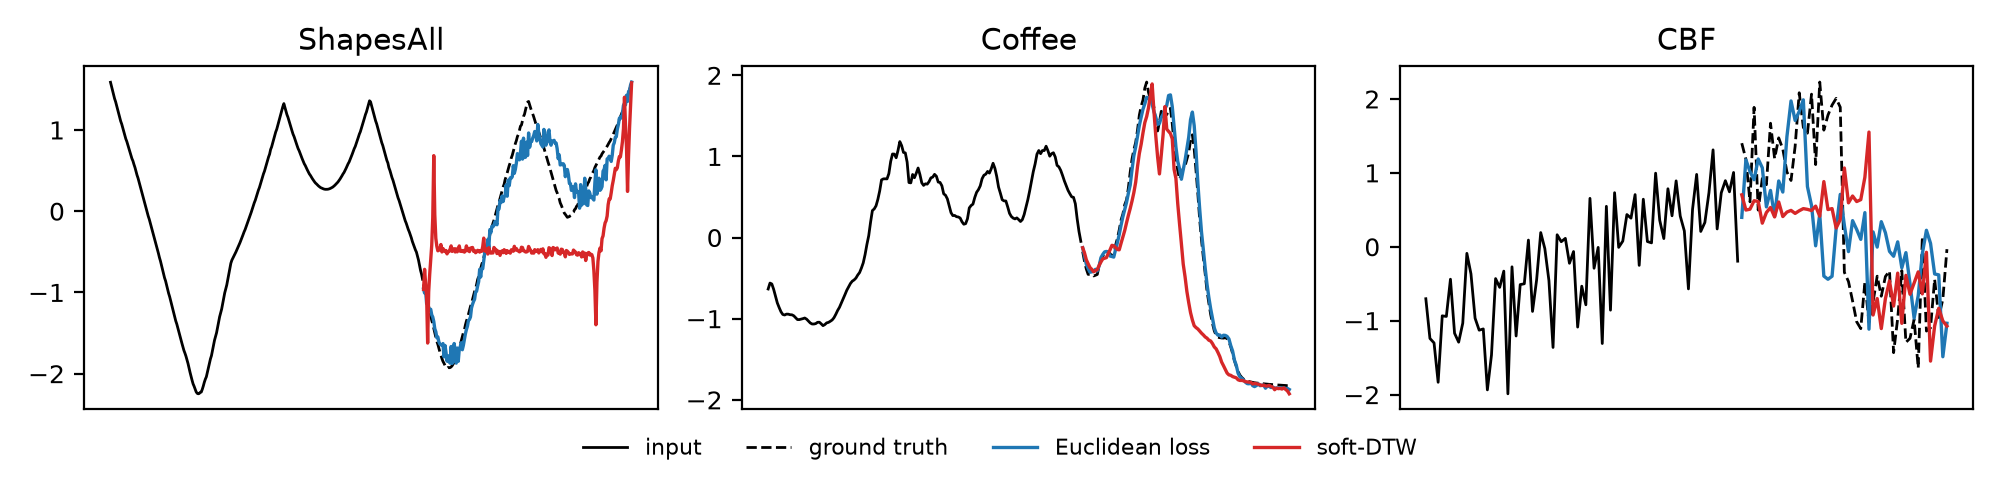
\includegraphics[width=\textwidth]{forecast_examples_slides.png}
\begin{block}{Why}
DTW can match one point of the prediction with a whole segment of the truth: \textbf{stretching time is free}, so one spike at the right height ``covers'' an entire rise.
\end{block}
\note{On ShapesAll, the dataset the paper uses to illustrate soft-DTW forecasting, our network trained from scratch predicts an almost flat line with spikes (red), yet its test DTW is lower than that of the Euclidean network (blue), which follows the truth much better. In DTW stretching time is free: one point can be matched with a whole segment. This is what our extension addresses.}
\end{frame}

% ----------------------------------------------------------------------
\section{Extension}
\begin{frame}{Soft-DTW$_\omega$: a penalty $\omega$ for every stretching step}
\begin{columns}[T]
\begin{column}{0.58\textwidth}
\[
r_{i,j}=\minop\{r_{i-1,j-1}+\delta_{i,j},\;r_{i-1,j}+\delta_{i,j}+\ours{\omega},\;r_{i,j-1}+\delta_{i,j}+\ours{\omega}\}
\]
\begin{itemize}
\item Cost of an alignment: $\langle A,\Delta\rangle+\omega\times(\#\text{stretching steps})$
\item Same $O(nm)$ forward and backward (soft DP with step costs, Mensch \& Blondel 2018)
\item $\partial/\partial\omega$ = expected number of stretching steps
\end{itemize}
\end{column}
\begin{column}{0.38\textwidth}
\centering
\begin{tabular}{ll}
\toprule
Limit & Recovers\\
\midrule
$\omega=0$ & soft-DTW\\
$\omega\to\infty$ & Euclidean distance\\
$\gamma\to0$ & amerced DTW\\
\bottomrule
\end{tabular}\\[0.1cm]
{\scriptsize Amerced DTW: Herrmann \& Webb, 2023.}\\[0.3cm]
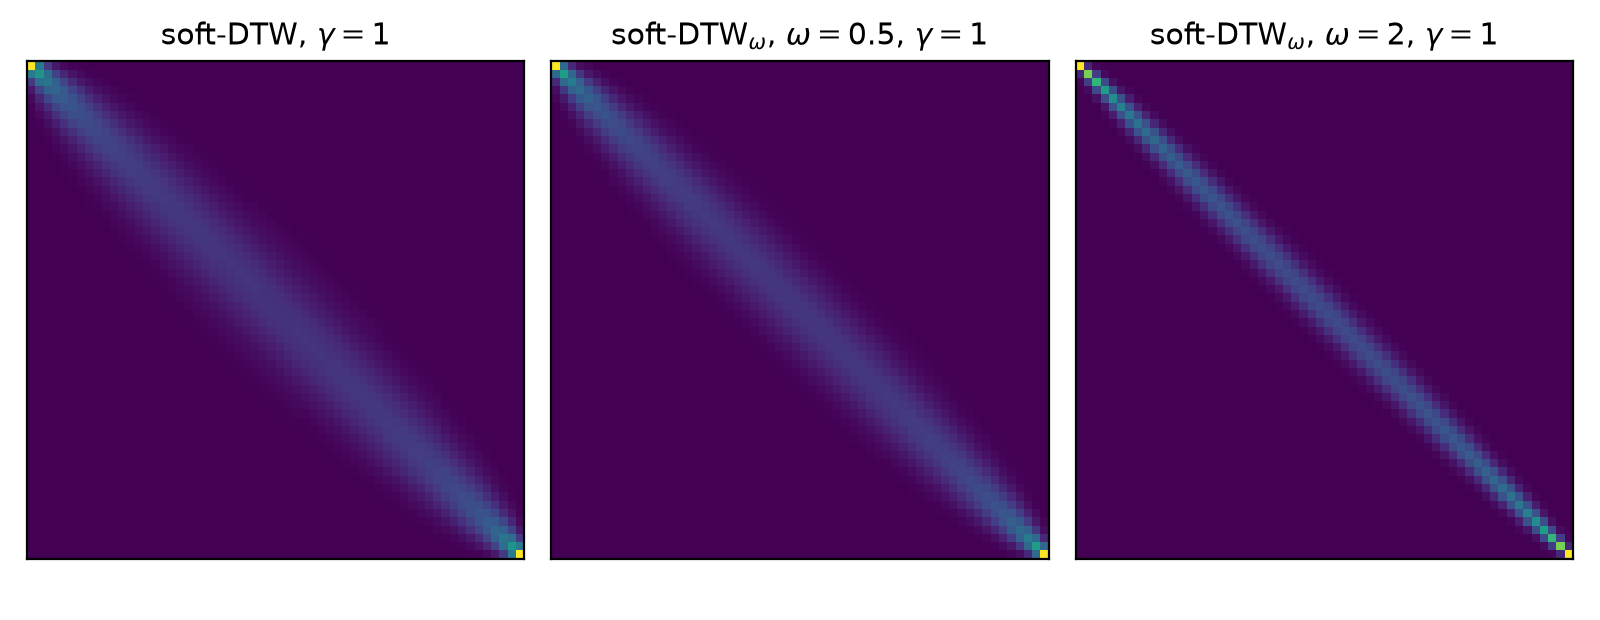
\includegraphics[width=\textwidth]{prior_zero_cost.png}\\
{\scriptsize $E$ with zero costs: the larger $\omega$, the less time is stretched.}
\end{column}
\end{columns}
\note{In soft-DTW the three steps entering a cell cost the same, so stretching time is free. We add a penalty omega to the two stretching steps. Omega zero gives soft-DTW, omega infinite only the diagonal (Euclidean distance), gamma to zero gives amerced DTW. Same O(nm) cost. It is a combination of existing ideas; what is new is using it as a smooth loss in the paper's experiments.}
\end{frame}

\begin{frame}{The penalty helps when the problem is getting lost}
\small
\begin{tabular}{p{0.33\textwidth}p{0.6\textwidth}}
\toprule
Experiment & Soft-DTW$_\omega$ vs soft-DTW (same $\gamma$, same start)\\
\midrule
Barycenters, random start & 8\% lower DTW loss, $1.3\times$ faster\\
Barycenters, Euclidean-mean start & Worse: DTW loss 7\% ($\omega=0.1$) to 30\% ($\omega=1$) higher. As $\gamma\to0$ it tends to DTW + $\omega$, not to the DTW loss used for scoring\\
$k$-means & Worse: DTW loss 10\% ($\omega=0.1$) to 50\% ($\omega=1$) higher\\
Nearest centroid & No gain: 0.85 vs 0.86 mean accuracy\\
Forecasting, from scratch & $\omega=0.1$: same DTW, 30\% lower Euclidean error. $\omega=1$: Euclidean error $\div$ 2 to 3 on all 13 datasets\\
\bottomrule
\end{tabular}
\vspace{0.5cm}
\begin{block}{}
$\omega$ pays off from a poor starting point (random weights, random barycenters), where free warping lets the optimisation fall into degenerate alignments. From a good start, plain soft-DTW is closer to what is measured.
\end{block}
\note{We added soft-DTW omega to every experiment, with the same draws and starting points. In forecasting from scratch it works very well. For barycenters from a random start it gives a lower loss and is faster. From a good start and in k-means plain soft-DTW is better, because the penalty changes the objective. In classification it makes no difference.

When we compute a barycenter (or train a network), the final DTW loss can be bad for two reasons. 1. Optimisation error: the method does not reach a good solution because it gets stuck in a bad minimum or in an absurd alignment. 2. Objective error: the method reaches the optimum of its own function, but that function is not exactly the one we measure, so its optimum is not the optimum of DTW. Omega reduces error 1, because it removes degenerate paths and makes the optimisation easier, but it adds error 2, because it optimises DTW plus omega and not DTW. The result depends on which of the two dominates. From a random start (random barycenters, networks trained from scratch) the main difficulty is not the objective but getting lost: bad local minima and degenerate alignments. The penalty removes those degenerate paths, and that gain is larger than the cost of the mismatch. From a good start (the Euclidean mean) there is no bad minimum to escape, so only the mismatch remains and plain soft-DTW, which tends exactly to DTW, wins. k-means suffers most because the penalty enters twice: in the centroids and in the assignment of every series to a cluster. In nearest centroid the score is the accuracy, not the DTW loss, and classification only needs the closest centroid to be the right one, so the mismatch barely matters. In forecasting the mismatch is visible too: with omega equal to 1 the test DTW is 6 to 9 percent worse, but from scratch the gain in stability and in Euclidean error is much larger.}
\end{frame}

% ----------------------------------------------------------------------
\section{Conclusion}
\begin{frame}{Conclusion}
\begin{columns}[T]
\begin{column}{0.32\textwidth}
\begin{block}{Reproduced}
Exact implementation (brute force, finite differences). The paper's four claims hold on our 10--13 datasets.
\end{block}
\end{column}
\begin{column}{0.32\textwidth}
\begin{block}{Nuanced}
Large gains only from poor starts; 14--16$\times$ DBA's cost at $\gamma=0.001$; unstable, degenerate forecasts from scratch.
\end{block}
\end{column}
\begin{column}{0.32\textwidth}
\begin{block}{Extended}
Soft-DTW$_\omega$ fixes the forecasting failures and trades shape for timing; it does not help from a good start.
\end{block}
\end{column}
\end{columns}
\vspace{0.5cm}
\textbf{Limitations.} $\omega$ is set by hand (minimising the loss itself drives $\omega\to0$, so it must be tuned on another objective) and depends on the scale of the costs; 13 datasets instead of 79.
\vspace{0.6cm}
\begin{center}
{\Large Thank you. Questions?}
\end{center}
\note{We re-implemented soft-DTW, verified it exactly, and the paper's claims hold. Magnitudes and costs nuance them. Our penalty fixes the forecasting failures but is not a better surrogate from a good start. Main limitation: omega is chosen by hand; learning it on the loss itself drives it to zero.}
\end{frame}

\end{document}
